% Template for ICME 2020 paper; to be used with:
%          spconf.sty  - ICASSP/ICIP/ICME LaTeX style file, and
%          IEEEbib.bst - IEEE bibliography style file.
% --------------------------------------------------------------------------
\documentclass{article}
\usepackage{spconf,amsmath,epsfig}
% \usepackage{svg}
\usepackage{float}

\let\OLDthebibliography\thebibliography
\renewcommand\thebibliography[1]{
  \OLDthebibliography{#1}
  \setlength{\parskip}{0pt}
  \setlength{\itemsep}{0pt plus 0.3ex}
}

\pagestyle{empty}


\begin{document}\sloppy

% % Example definitions.
% % --------------------
% \def\x{{\mathbf x}}
% \def\L{{\cal L}}


% Title.
% ------
\title{Chatroom Project}
%
% Single address.
% ---------------
\name{Gerard (Jed) Mijares, Andrew Perry}
%Address and e-mail should NOT be added in the submission paper. They should be present only in the camera ready paper. 
\address{}


\maketitle


%
\begin{abstract}
% The abstract should appear at the top of the left-hand column of text, about 0.5 inch (12 mm) below the title area and no more than 3.125 inches (80 mm) in length.  Leave a 0.5 inch (12 mm) space between the end of the abstract and the beginning of the main text.  The abstract should contain about 100 to 150 words, and should be identical to the abstract text submitted electronically along with the paper cover sheet.  All manuscripts must be in English, printed in black ink.

A critical function of the internet has always been allowing people to communicate with each other remotely. This has been especially relevant this year, as it is more difficult to meet with people in person as a result of the COVID-19 pandemic. Due to this, the group decided to create a chatroom application to explore this area firsthand. 

\end{abstract}
%
% \begin{keywords}
% One, two, three, four, five
% \end{keywords}
%
\section{Introduction}
\label{sec:intro}

% \subsection{Abstract}

\subsection{Relevance to the Course}

The project most heavily builds on the content in Chapter 2 of Kurose's textbook, \emph{Computer Networking} \cite{kurose}. Specifically, the topics that were used are programming with sockets and sending messages or files back and forth. 

This project also relates to the material from Chapter 8 \cite{kurose}. These topics are security and end-to-end encryption. 

Getting experience with these concepts helped to understand and reinforce the real-world applications where they are used. For example, seeing the effect that no encryption has on the security of the messages. Without any security, the messages could be easily intercepted and read with a packet sniffer such as Wireshark. We found that programming and using these techniques first-hand reinforces the concepts.

\begin{figure}[h]
\caption{Demonstration of clients chatting via our chatroom application.}
\centering
\includegraphics[width=0.5\textwidth]{media/usersChatting.PNG}
\label{usersChatting}
\end{figure}

\section{Literature Review}

\subsection{Comparison to Internet Relay Chat (IRC)}

% \begin{figure}[h]
% \caption{Client/Server Network Architecture Diagram. Image from \cite{pic_from_wiki}.}
% \centering
% \includegraphics[width=0.5\textwidth]{media/Network.PNG}
% \label{Network Architecture}
% \end{figure}

Internet Relay Chat (IRC), an open internet chatting protocol, was invented in 1988 \cite{radwareIRC} and is the largest inspiration for our application. Although more robust chatroom applications, discussed in section 2.2, have gained popularity among internet users, IRC still retains a number of dedicated users to this day.

Similar to our protocol, it operates on a client server scheme. As the protocol is "open", anybody who properly implements the protocol can connect to or create a server. 

Our protocol adds some features present in proprietary chat applications that are not available in "vanilla" IRC (Though some users have created custom IRC extensions or clients that add similar functions \cite{whatsIRC}).

% Other open chat examples are XMPP and PSYC. 

\subsection{Comparison to Proprietary Applications}

Services such as Slack or Discord are products that also offer chat applications. These applications are often robust and offer a greater amount of features, sometimes catering to a certain target market. For example, Slack is geared towards a professional work environment \cite{slack} while Discord offers features appealing to video game enthusiasts \cite{discord}. We chose to implement some of the features these platforms offer into our protocol.

Unlike IRC and the chatroom application created for this project, these proprietary applications offer a standard client to use their service. It is often not possible (or otherwise inconvenient, due to restrictions placed by the service \cite{discordTweet}) to create a custom client to connect to these applications. However, some may offer Application Programming Interfaces (APIs) for developer's to create some sort of interface with the service, such as bots \cite{discordDev}. 

\subsection{Types of Encryption}

Encryption is a necessary aspect of chatroom applications, one that developers must keep in mind while creating applications. Without sufficient encryption, malicious onlookers will not only have the potential to read messages sent between users, but also to obtain personal information, such as passwords. One key aspect of our project is to begin developing our chatroom's encryption methods, beginning with the encryption of chat messages. 

One of the most trusted encryption techniques is the Advanced Encryption Standard (AES). AES is the encryption standard used by the United States government\cite{US_gov_encryption}, banks, and many other corporations where encryption is massively important. One pro of AES are its use of "symmetric encryption"\cite{Encryption_Types}, meaning that the same key that is used for encryption is also used for decryption. Another pro is that the large key sizes used by AES (supports 128, 192, and 256 bits) makes hacking encrypted data virtually impossible. The con of this method, however, is that AES encrypts in blocks of 128 bits, which can lead to a time consuming and memory intensive encryption and decryption process for very large files. 

Since text messages make up the majority of communication in our chatroom application, the pros of robust security and simple implementation outweigh the cons of time and memory intensiveness. 

Other options that were considered for this project were Salsa20 and Data Encryption Standard (DES)\cite{DES_info}. Both of these options were quickly ruled out in favor of AES. While Salsa20 has the potential to provide faster encryption times on large files, its use is not near as documented and established as AES. DES is a more well known encryption standard, but its short key length of 56 bits makes it much easier to crack. 

More information on AES and other encryption types can be found in ~\cite{encryption}.

\subsection{Architecture Options}

We explored two options for our chatroom network architecture: the server-client model or peer-to-peer (P2P). In this section, the pros and cons of each is discussed, and one is selected for our project. 

% Probably shouldn't make these claims without sources
% The client-server model is the most obvious option for our chatroom application. This is because client-server is used by nearly all chatroom applications. IRC, the first popularized chatroom application, used the client-server model shown in Figure \ref{Network Architecture}, and all of the proprietary applications mentioned in Section 2.2 make use of the client-server model. This is because the client-server model has many pros that make it ideal for these applications. Some examples are: 

The first model we had considered was the client-server model. This model lends itself well to a chatroom application, and is the model used by IRC \cite{IRCmemo} and other protocols. It offers several advantages relevant to this type of application, such as:

\begin{itemize}
  \item easy control of servers, as programs or clients cannot easily damage the system
  \item easy to maintenance servers as clients are not involved in the process
  \item ease to add more nodes to the network.
\end{itemize}

This architecture still has drawbacks. These include performance dips as the number of clients increase and potential for chatroom failure if one or more servers fail.~\cite{clientserver} gives additional info on the pros and cons of the client-server architecture.

Peer-to-peer (P2P) is an architecture that is not as commonly used for chatroom applications, but is still very popular. P2P is often used for file sharing applications, with the most notable protocol being BitTorrent. The pros of P2P include not needing to create and maintain expensive servers since the application is run on the client's device, and the failure of a single client will not lead to the destruction of the network, since each client is only a bit of the connection. (This is opposed to client-server, where the crashing of a server could have disastrous results.) A key downside to P2P is lower security, since clients have much more control over the workings of the program. More details on the P2P architecture can be found in~\cite{P2P}.

After researching this info, we decided to base our chatroom on a client-server model. This is because the client-server model allows for a higher degree of security when sending messages, and our chatroom will be operating on a small scale, so the key downside of the client-server model will not harm the chatroom performance. In order to keep the project from getting too complex, and to create a unique chatroom application from IRC, we decided to also send files over the client-server architecture as well.

\section{Technical Approach Description}

\subsection{Threaded Chat Program}

At first, we approached the challenge with a simple procedural program on each end of the chatroom. We quickly found this was insufficient - users could indeed communicate with each other, but only if they took turns sending messages to each other. Otherwise the program would hang, not allowing the user to continue to send messages until they had received one.

To solve the problem, we redirected the chatroom program using a multi-threaded approach for both the client and server.

\begin{figure}[h]
\caption{Beginning of Server Code}
\centering
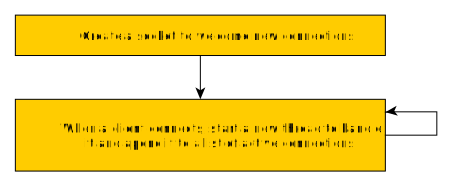
\includegraphics[width=0.5\textwidth]{media/serverFlowchart2.png}
\label{server2}
\end{figure}

When the user decides to create a new server on their device, the program first creates a socket to handle new connections, then waits for clients to connect, as demonstrated in Figure \ref{server2}.

\begin{figure}[h]
\caption{Server code to connect to each client}
\centering
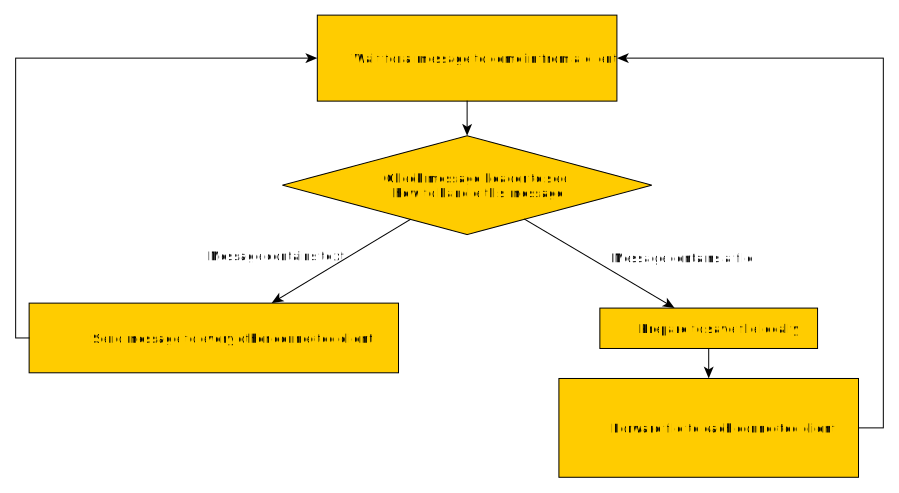
\includegraphics[width=0.5\textwidth]{media/serverFlowchart1.png}
\label{server1}
\end{figure}

When a client connects, the server creates a new thread to run the code loop demonstrated in Figure \ref{server1}. The object running this thread is appended to a list of active client connections. When a message is sent from the server, the server will go through this list and forward the message to each client.

\begin{figure}[h]
\caption{Code running at beginning of Client Program}
\centering
\includegraphics[width=0.5\textwidth]{media/clientFlowchart2.png}
\label{client2}
\end{figure}

When the user decides to connect to a server as a client, the code described in Figure \ref{client2} is run. First, the user is prompted for information including the IP address of the server they are connecting to, the username they would like to use, and the encryption key they will use. Then, two threads are created, one to handle sending and one for receiving.

\begin{figure}[h]
\caption{Code loop to handle sending messages to the server}
\centering
\includegraphics[width=0.5\textwidth]{media/clientFlowchart1.png}
\label{client1}
\end{figure}

Figure \ref{client1} gives an overview of the code facilitating the sending of messages from client to server. The program waits for input from the user, and when a message is entered, it checks for a command at the beginning of the message. Currently, the only command available is "!send" to send a file, but other commands could be implemented in the future as well. If no command is present, then the message is encrypted and sent to the server.

\begin{figure}[h]
\caption{Client code to receive messages from the server}
\centering
\includegraphics[width=0.5\textwidth]{media/clientFlowchart3.png}
\label{client3}
\end{figure}

Finally, the code describing the receiving of messages is described in Figure \ref{client3}. Each client will wait for a message to arrive from the server, and will then check the messages header to determine what kind of processing is required. For a text message, that is decrypting the message and printing it to the screen, and for a sent file, that is parsing the filename and writing the file itself to that file.

\subsection{Encryption}

After the selection process for encryption types discussed in section 2.3, we decided to implement a form of AES encryption. There are many Python libraries that implement this exact architecture, many operating in similar ways. We decided to use the Fernet library in Python's Cryptography suite. 

When a client first connects to a server, they are asked to provide an encryption key, as shown in Figure 7. Since AES uses symmetrical encryption, this is the key that will be used to both encrypt outgoing messages and decrypt incoming messages. Clients will be able to communicate successfully only if they have already agreed on a key beforehand. If the key is misplaced somehow, the two will only be able to communicate after agreeing on another key via a separate channel.

After a client has connected, the key that they input will be used to encrypt and decrypt. If two clients have entered equivalent keys, then their messages will be successfully transferred. If a client attempts to decode a message with a different key, the decryption function will fail, and the message "ERROR: ENCRYPTION KEY IS DIFFERENT" will show instead of the intended message. 

The only complication in this method occurred on the decryption side. When a client-inputted message is encrypted, the encrypted message is contained as a bit string. This encrypted message is received as a string on the receiving end. This string had to be casted back to a bit string in order to work with the Fernet decryption function.

\begin{figure}[h]
\caption{The client is asked for an IP, username and encryption key before connecting to the server.}
\centering
\includegraphics[width=0.5\textwidth]{media/StartCode.PNG}
\label{client3}
\end{figure}

\subsection{File Sharing}

As mentioned previously, the user may send a file located on their device with "!send \emph{filename}". When this occurs, the client first sends a short message with the header "FILE" (as opposed to the "TEXT" of a general chat message). This initial message contains the file's name and its size. After sending this message, the client begins sending the file sequentially, until the entire file has been sent. This process is shown in Figure \ref{client1}.

When the server receives the "FILE" header message, it first parses the given file name and size. Then, it opens a file with the given file name and begins to write the data sent from the client into that file. Once complete, it sends the file to each connected client, just as the client sent it to the server. This process is shown in Figure \ref{server1}.

Finally, the receiving clients receives the "FILE" message and file data from the server, as shown in Figure \ref{client3}. The user is able to use the file as they wish. A practical use of this feature is shown in Figure \ref{fileshareDemo}.

\begin{figure}[h]
\centering
\caption{Demonstration of filesharing application}
\includegraphics[width=0.5\textwidth]{media/fileshareDemo.png}
\label{fileshareDemo}
\end{figure}

Unlike text messages, files are not currently encrypted. Other potential improvements to this feature that could be added in the future include error handling if a file is not present, parallelizing the sending of the file, and automatically displaying the file in the receiver's default application for the given file type.

\section{Experimental Results and Discussion}

\subsection{Encryption}

\begin{figure}[h]
\centering
\caption{Results of the first experiment to show the effectiveness of encryption.}
\includegraphics[width=0.5\textwidth]{media/EncryptionExperiment.PNG}
\label{Encryption Results Figure}
\end{figure}

\begin{figure}[h]
\centering
\caption{Results of Encryption on Legibility of Wireshark Captures. The capture on the top is from an encrypted message, while the capture on the bottom is from a non-encrypted message. The capture on the top is illegible, while the non-encrypted capture can be read directly.}
\includegraphics[width=0.5\textwidth]{media/WiresharkEncryptionResults1.PNG}
\includegraphics[width=0.5\textwidth]{media/WiresharkEncryptionResults2.PNG}
\label{Encryption Wireshark Results}
\end{figure}

Two tests were run to make sure that the encryption method was actually working. First, the effectiveness of encryption was shown in the chatroom itself. To make sure that the encryption method actually prevented users with different encryption keys from viewing each other's messages, three clients were connected to a server. Two of these clients have equivalent encryption keys, while the third user has a different key. If the encryption method works correctly, the two users with equivalent keys will be able to read each other's messages, while the third user will only see the error message described in section 3.2. Similarly, the two users should not be able to read the messages from the third user with a different key. 

The results of this experiment are shown in Figure \ref{Encryption Results Figure}. The clients with usernames "Andrew" and "Jed" both have the same encryption key, while "Random guy" has a different key. As expected, the users Andrew and Jed were able to read each other's messages, while Random guy could only see an error code. Additionally, users Andrew and Jed could not read the messages that Random guy sent. 

The purpose of the second experiment is to prove that the encryption is disabling others from being able to intercept the messages. To prove this, Wireshark was used to intercept message packets. These captured packets are shown in Figure \ref{Encryption Wireshark Results}. The top packet is a capture from an encrypted message, while the bottom capture is from a non-encrypted message. Because of encryption, the message at the top is unreadable. There is no hint of the original message contents in the packet. The message contents from the bottom packet, on the other hand, can be read plainly. 

Both of these experiments prove that the encryption mechanism not only prevents unintended clients from reading messages from other clients, but also that the encryption method prevents packet sniffers such as Wireshark from being able to read the contents of messages. 

\subsection{File Sharing}
We found we were successfully able to send files from one computer to another. However, we noticed that the received files occasionally had slight errors in transmission. For example, pictures might send, but have a small gray rectangle near the bottom. It seems something in the code may have been cutting off the transmission early for larger files, but we were not able to fully debug this issue. So, while this application may be sufficient casual sending of files such as images and text documents, it can fail for more complex files. Improving this feature is one possible development that could be done at a later date.

% \section{Discussions on Results}

\section{Division of Labor}

The division of labor is as follows.

Jed:
\begin{itemize}
  \item Multi-threaded chat program
  \item File transfer
  \item Code flowcharts
\end{itemize}

Andrew: 
\begin{itemize}
  \item Encryption
  \item Encryption Wireshark experiment. 
\end{itemize}

Both worked together on team items, such as the report and presentation.

\section{Conclusion}

To summarize, the project successfully completed all of our goals. We created a TCP chatroom program allowing multiple users to communicate with each other remotely and securely, as well as share files. The research that guided this process is detailed in section 2, and the technical details of the project are described in section 3. In section 4, encryption and file sharing were tested to display how they function. 

There is still room to expand on this project. Given more time, the next set of objectives would be as follows: 
\begin{itemize}
  \item Caching messages
  \item Private messages
  \item Improving robustness/error handling
  \item Improved user interface
  \item Encryption/decryption of files
\end{itemize}

% References should be produced using the bibtex program from suitable
% BiBTeX files (here: strings, refs, manuals). The IEEEbib.bst bibliography
% style file from IEEE produces unsorted bibliography list.
% -------------------------------------------------------------------------
\bibliographystyle{IEEEbib}
\bibliography{icme2020template}

\end{document}
